\documentclass[12pt,letterpaper]{article}
\usepackage{graphicx,textcomp}
\usepackage{natbib}
\usepackage{setspace}
\usepackage{fullpage}
\usepackage{color}
\usepackage[reqno]{amsmath}
\usepackage{amsthm}
\usepackage{fancyvrb}
\usepackage{amssymb,enumerate}
\usepackage[all]{xy}
\usepackage{endnotes}
\usepackage{lscape}
\newtheorem{com}{Comment}
\usepackage{float}
\usepackage{hyperref}
\newtheorem{lem} {Lemma}
\newtheorem{prop}{Proposition}
\newtheorem{thm}{Theorem}
\newtheorem{defn}{Definition}
\newtheorem{cor}{Corollary}
\newtheorem{obs}{Observation}
\usepackage[compact]{titlesec}
\usepackage{dcolumn}
\usepackage{tikz}
\usetikzlibrary{arrows}
\usepackage{multirow}
\usepackage{xcolor}
\newcolumntype{.}{D{.}{.}{-1}}
\newcolumntype{d}[1]{D{.}{.}{#1}}
\definecolor{light-gray}{gray}{0.65}
\usepackage{url}
\usepackage{listings}
\usepackage{color}
\UseRawInputEncoding

\definecolor{codegreen}{rgb}{0,0.6,0}
\definecolor{codegray}{rgb}{0.5,0.5,0.5}
\definecolor{codepurple}{rgb}{0.58,0,0.82}
\definecolor{backcolour}{rgb}{0.95,0.95,0.92}

\lstdefinestyle{mystyle}{
	backgroundcolor=\color{backcolour},   
	commentstyle=\color{codegreen},
	keywordstyle=\color{magenta},
	numberstyle=\tiny\color{codegray},
	stringstyle=\color{codepurple},
	basicstyle=\footnotesize,
	breakatwhitespace=false,         
	breaklines=true,                 
	captionpos=b,                    
	keepspaces=true,                 
	numbers=left,                    
	numbersep=5pt,                  
	showspaces=false,                
	showstringspaces=false,
	showtabs=false,                  
	tabsize=2
}
\lstset{style=mystyle}
\newcommand{\Sref}[1]{Section~\ref{#1}}
\newtheorem{hyp}{Hypothesis}

\title{Final Project - Data Visualisation for Social Scientists}
\date{Due: March 8, 2026}
\author{Matilda Tomatis}

\begin{document}
	
	\maketitle
	\tableofcontents
	\newpage
	
	\section{Executive Summary}
	
\vspace{0.5cm}
	
\noindent This report investigates whether female cabinet members in the 38 OECD countries are more left-leaning in their ideological positioning than their male counterparts.

\noindent The analysis uses data from the \emph{Manifesto Project} and the \emph{WhoGov} datasets, which provide information on the country, year, gender, and party affiliation of cabinet members.

\noindent To examine potential gender differences in ideology, the report analyses the relationship between the share of women in cabinets and the average ideological position of cabinets. It also presents yearly boxplots comparing the ideological positioning of female and male ministers, as well as a heatmap of the gender gap in cabinet ideology.

\noindent The results do not provide strong evidence supporting the hypothesis that female ministers are systematically more left-leaning than male ministers.

\vspace{0.5cm}
	
	\section{Data Background \& Hypothesis}
	
\vspace{1cm}

\noindent The analysis proposed investigates whether female politicians tend to be more left-leaning than their male counterparts. It is a widely investigated, and often implicitly assumed, topic in political science \emph{(Van Der Pas \& Aaldering, 2022)}. Moreover, the pattern seems to hold within both right-wing and left-wing parties \emph{(De Geus \& Shorrock, 2020)}: even female right-wing politicians tend to position themselves more to the left than their male counterparts.

\noindent Based on these findings, the analysis tests the following hypothesis: 
\begin{center}
	\textbf{H:} \textit{Female politicians are, on average, more left-leaning than their male counterparts.}
\end{center}

\vspace{0.5cm}
\noindent The analysis uses a panel time series dataset spanning over 30 years (from 1990 to 2023) for the 38 members of the Organisation for Economic Co-operation and Development [OECD]. More in particular, data from the \href{https://manifesto-project.wzb.eu/}{Manifesto Project Database} and from the \href{https://politicscentre.nuffield.ox.ac.uk/whogov-dataset/}{WhoGov Dataset} are employed to obtain information about the \textbf{sex and party affiliation} of the ministers in each country-year combination, as well as their \textbf{right-left positioning on the ideological spectrum}.

\noindent \textbf{The Manifesto Project Dataset} uses quantitative content analysis methods on parties' election manifestos to study parties' policy preferences; thereafter positioning them on a left-right political spectrum. Lower values indicate left-leaning ideologies, while positive values indicate right-wing parties.  

\noindent \textbf{The WhoGov Dataset} provides bibliographic information, such as the aforementioned gender and party affiliation, of cabinet members; as well as information on the duration and type of government in place. 

\section{Data Cleaning}
\noindent As anticipated, all 38 OECD countries are selected for the analysis. This choice leads to an unbalanced panel dataset. 
\vspace{0.5cm}

\lstinputlisting[language=R, firstline=36, lastline=44]{final_MT.R}

\vspace{0.5cm}
\noindent From the Manifesto Project dataset, the variables \emph{edate, countryname, rile and partyname} were subselected, filtering the observations for the years 1990 to 2023 and for the selected countries. Considering that the dataset contains information on parties only for election years, the positioning (RILE) was artificially carried forward to the non-election years without available data. 

\noindent Both the WhoGov \textbf{within-country} and \emph{cross-sectional} datasets were employed. In the first, the variables \emph{country\_name, year, name, gender, minister and party\_name} are retained; in the cross-sectional dataset, the columns \emph{country\_name, year, n\_female\_minister and n\_minister} are subselected. Both datasets are filtered for the selected countries and the same time interval as before. In substance, only observations related to ministers were kept and are analysed in this project. 

\noindent The cleaning and wrangling of the datasets was quite labourious, mainly because of some incongruences in the English names of the ministers' national parties of affiliation in the WhoGov and Manifesto Project datasets. Therefore, the party names were cleaned and standardised; a matching (or partial matching) procedure was then performed when merging the two datasets. The final dataset \textbf{WG\_within\_rile} includes the ministers’ names, their gender, their party of affiliation, whether they were cabinet ministers, and their left-right ideological positioning (based on the party of affiliation).  

\noindent Additionally, the dataset \textbf{WG\_cross} is created, containing the variables year, country, and the share of female ministers (i.e.\ the number of female ministers divided by the total number of ministers); and the dataset \textbf{WG\_rile\_avg}, which includes year, country, and the average left-right ideological positioning. 

\noindent It is very important to note that for some parties, especially smaller parties or recently created ones, the \emph{RILE} score is not present; thereof, NAs replace it. The computation of some of the statistics might be compromised for some country-year combinations because of this issue. 


\vspace{0.5cm}
\noindent To assure a more cohesive style of the visualisation, a ggplot theme is created for this project.
\vspace{0.5cm}

\lstinputlisting[language=R, firstline=217, lastline=229]{final_MT.R}

	\section{Analysis}
		\subsection{Female Ministers Share \& Left-Right Positioning}
		
\vspace{0.5cm}
\noindent One way in which the hypothesis is tested is by verifying whether the increasing presence of female politicians in cabinets occurs when a country’s government has, on average, a more left-leaning ideology. 

\noindent To visualise this assumption, a line graph of the share of female ministers (\emph{n\_female\_minister / n\_minister}) over time is plotted for each of the OECD countries. Additionally, the OECD average is reported. 

\vspace{0.5cm}
\lstinputlisting[language=R, firstline=234, lastline=251]{final_MT.R}

\begin{figure}[H]\centering
	\caption{}
	\label{fig:visualisation_1}
	\hspace*{-1.5cm}
	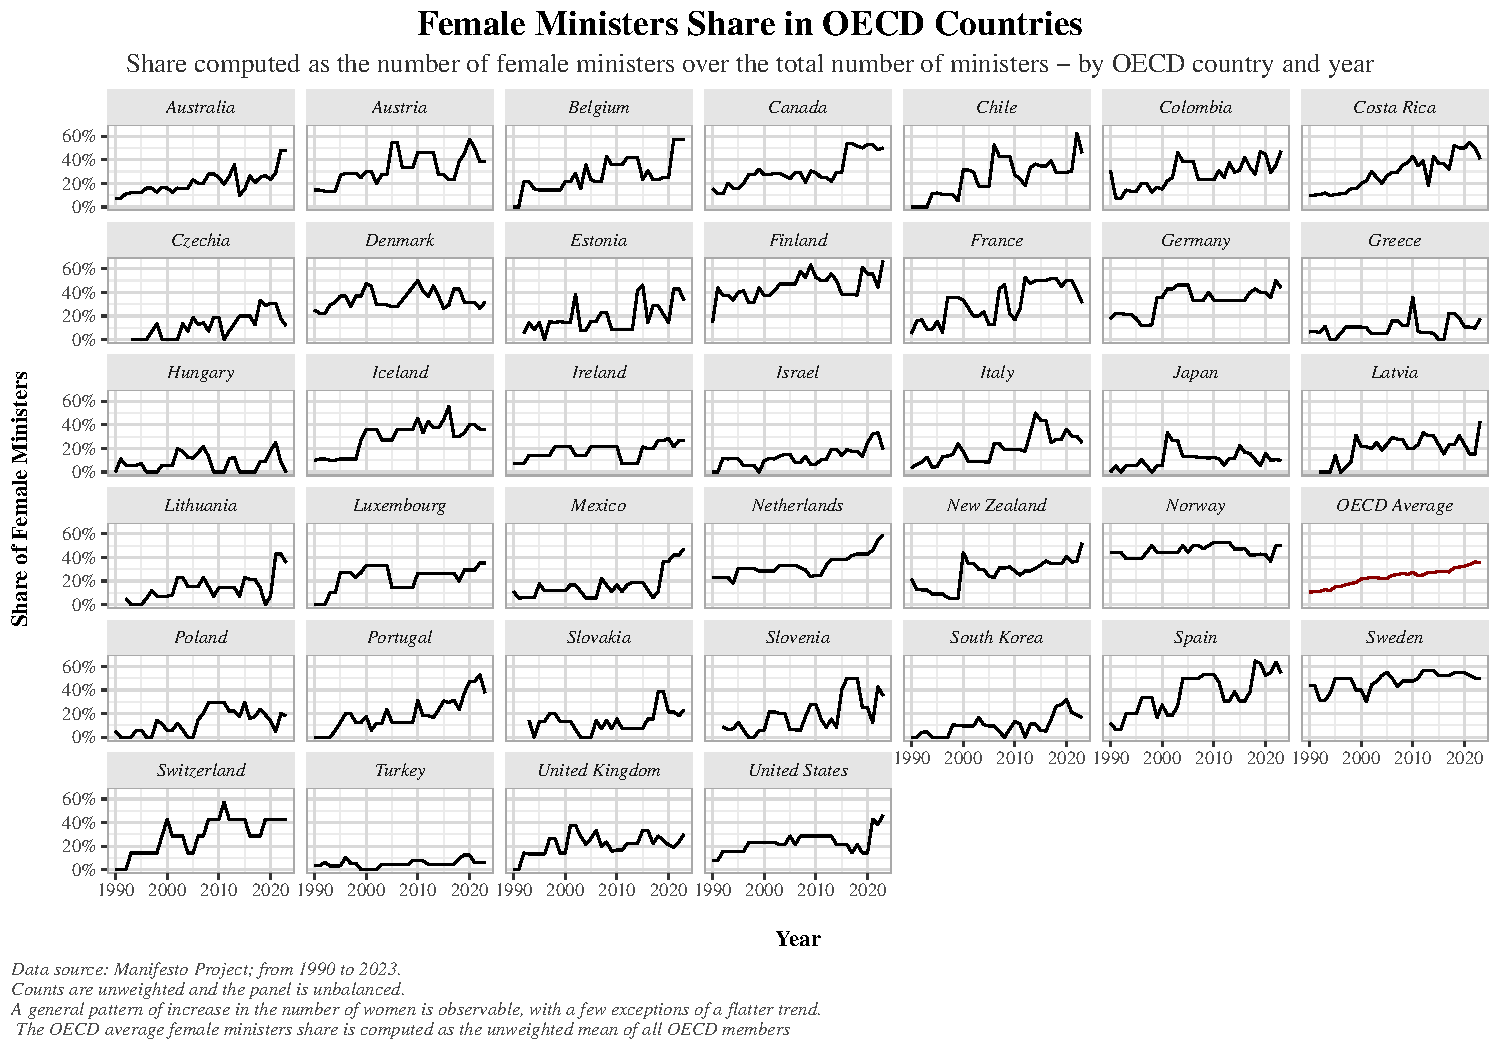
\includegraphics[width=1.1\textwidth]{linegraph_share.pdf}
\end{figure}

\vspace{0.5cm}
\noindent The same procedure is repeated for the average left-right ideological positioning of cabinets (computed as the mean \emph{RILE} score). 

\vspace{0.5cm}
\lstinputlisting[language=R, firstline=378, lastline=395]{final_MT.R}

\begin{figure}[H]\centering
	\caption{}
	\label{fig:visualisation_2}
	\hspace*{-1.5cm}
	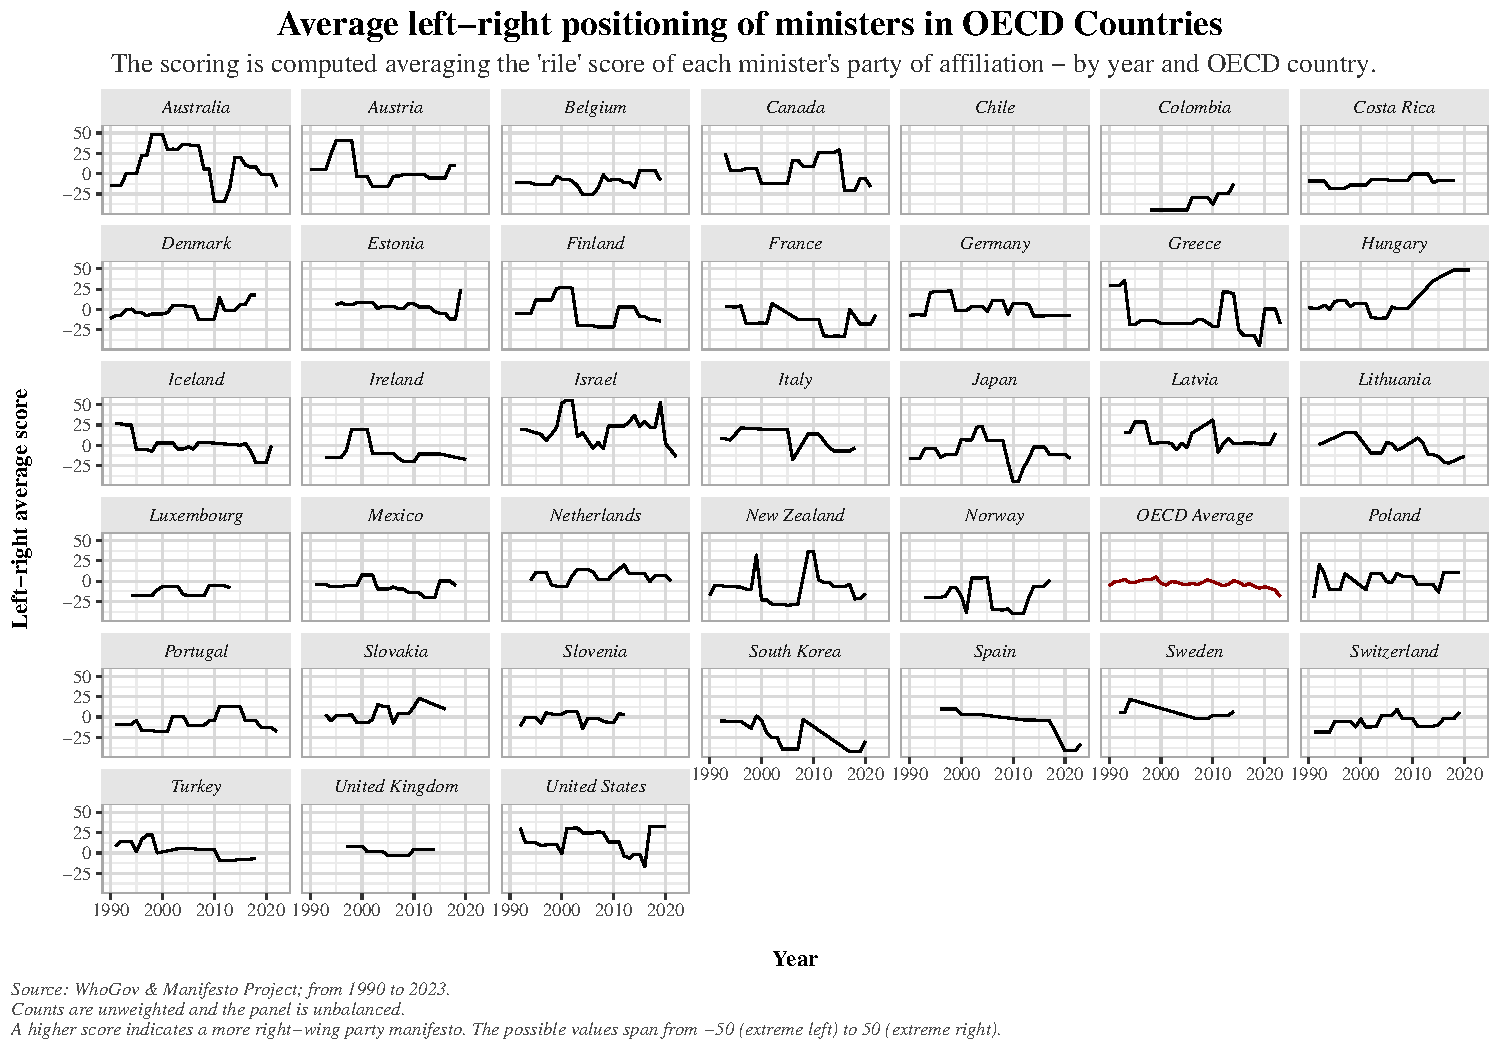
\includegraphics[width=1.1\textwidth]{linegraph_rile.pdf}
\end{figure}

\vspace{0.5cm}
\noindent To further investigate the possible link between the share of female ministers and the left-right positioning of cabinets, quartiles are computed for both \emph{avg\_rile} and \emph{fem\_min\_share}. Countries are then assigned to each quartile and mapped accordingly; these visualisations allow us to visually check whether countries move across quartiles simultaneously. 

\noindent For the figures, quartiles were computed and the maps were generated every 10 years (i.e., 1990, 2000, 2010, and 2020). For better space usage, only the code for one of the four year-specific maps is reported. 

\vspace{0.5cm}
\lstinputlisting[language=R, firstline=256, lastline=285]{final_MT.R}
\lstinputlisting[language=R, firstline=353, lastline=362]{final_MT.R}

\begin{figure}[H]\centering
	\caption{}
	\label{fig:visualisation_3}
	\hspace*{-1cm}
	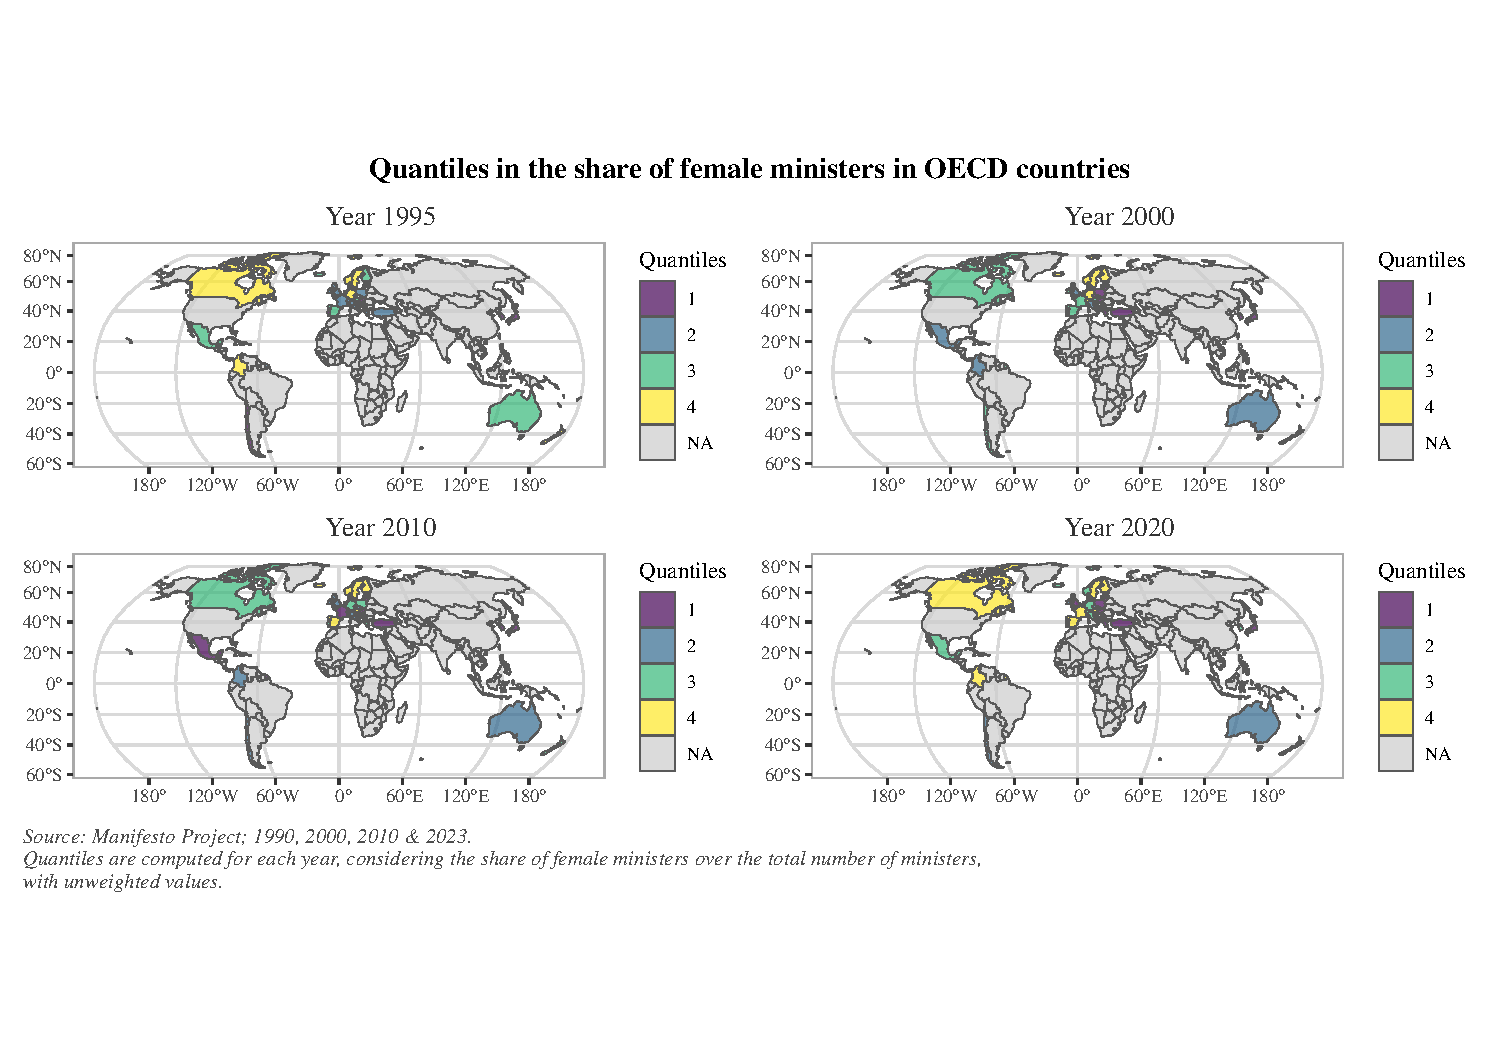
\includegraphics[width=1.1\textwidth]{wm_9020_share.pdf}
\end{figure}

\vspace{0.5cm}
\lstinputlisting[language=R, firstline=402, lastline=420]{final_MT.R}
\lstinputlisting[language=R, firstline=488, lastline=497]{final_MT.R}

\begin{figure}[H]\centering
	\caption{}
	\label{fig:visualisation_4}
	\hspace*{-1cm}
	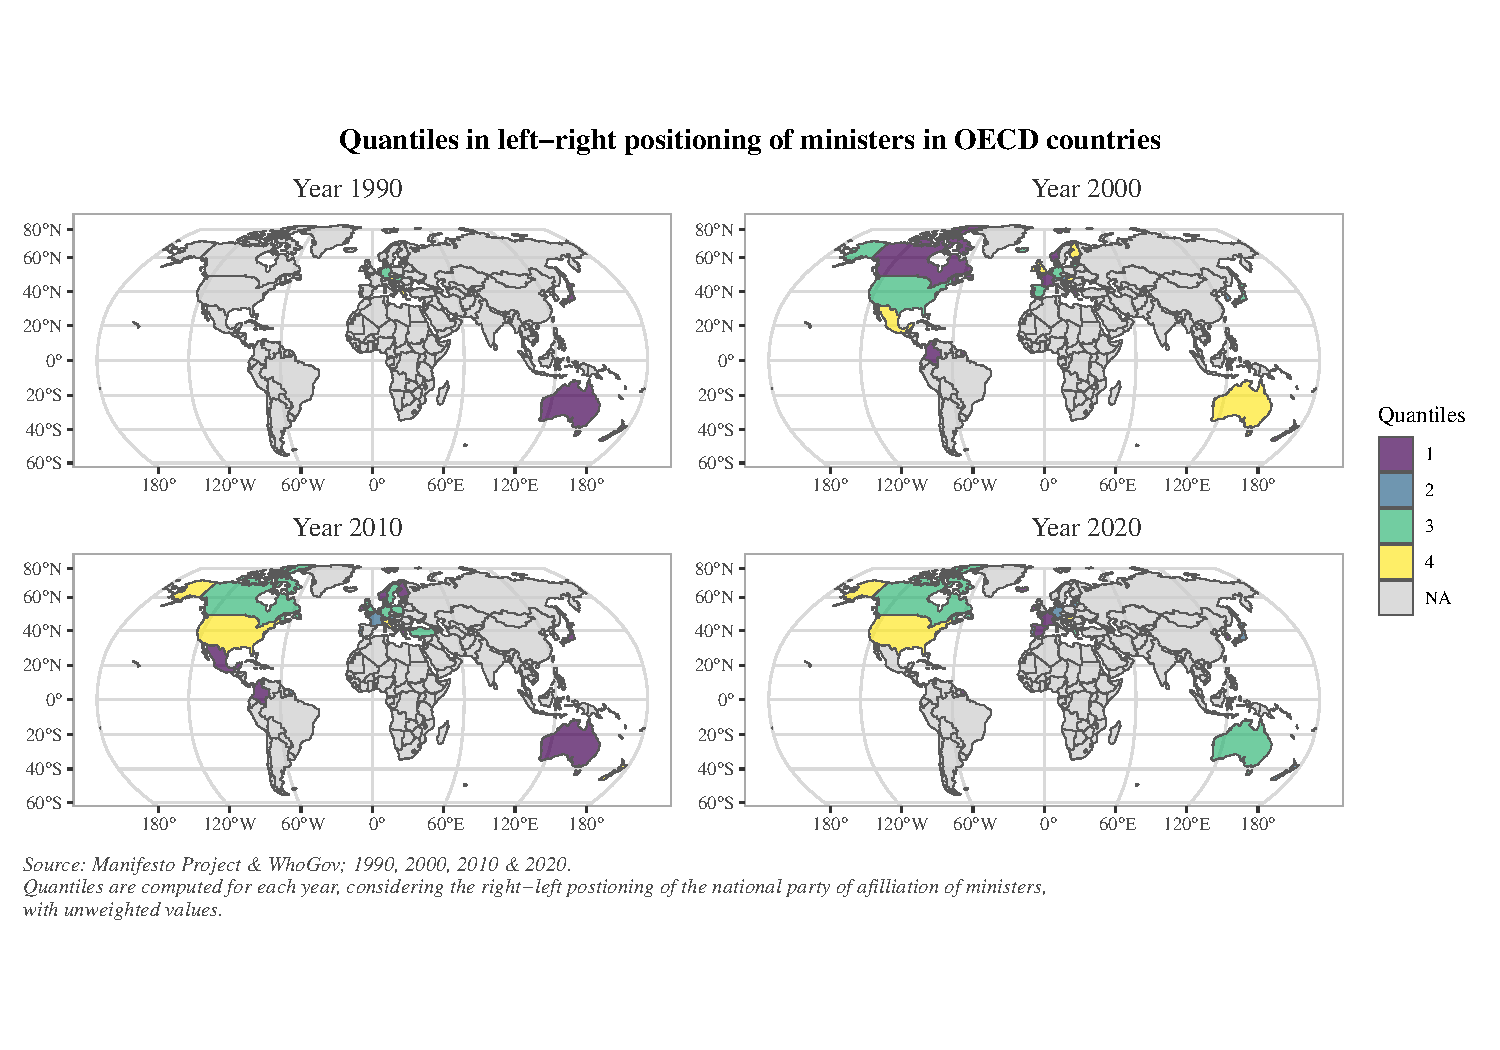
\includegraphics[width=1.1\textwidth]{wm_9020_rile.pdf}
\end{figure}

\vspace{0.5cm}
\noindent According to our hypothesis, higher quantiles in Figure 3 should correspond to lower quartiles in Figure 4, and vice versa. While the two quartiles occasionally move together, there is no consistent pattern of synchronized movement. This evidence suggests weak to no support for the initial hypothesis.

\vspace{0.5cm}
	\subsection{Boxplot of Female and Men Ministers' Ideological Positioning}

\vspace{0.5cm}
\noindent Afterwards, to investigate the hypothesis using another approach, two boxplots presenting the ideology of the whole sample of women and the whole sample of men are plotted. Once again, it was decided to replicate the plots for four selected years (1990, 2000, 2010, and 2020) in order to verify whether the possible differences are consistent over time. 

\noindent This approach allows for a different perspective from the previous analysis, no longer relating the number of female ministers to the average ideology of the country, but instead considering individual observations.

\vspace{0.5cm}
\lstinputlisting[language=R, firstline=506, lastline=525]{final_MT.R}

\begin{figure}[H]\centering
	\caption{}
	\label{fig:visualisation_5}
	\hspace*{-1cm}
	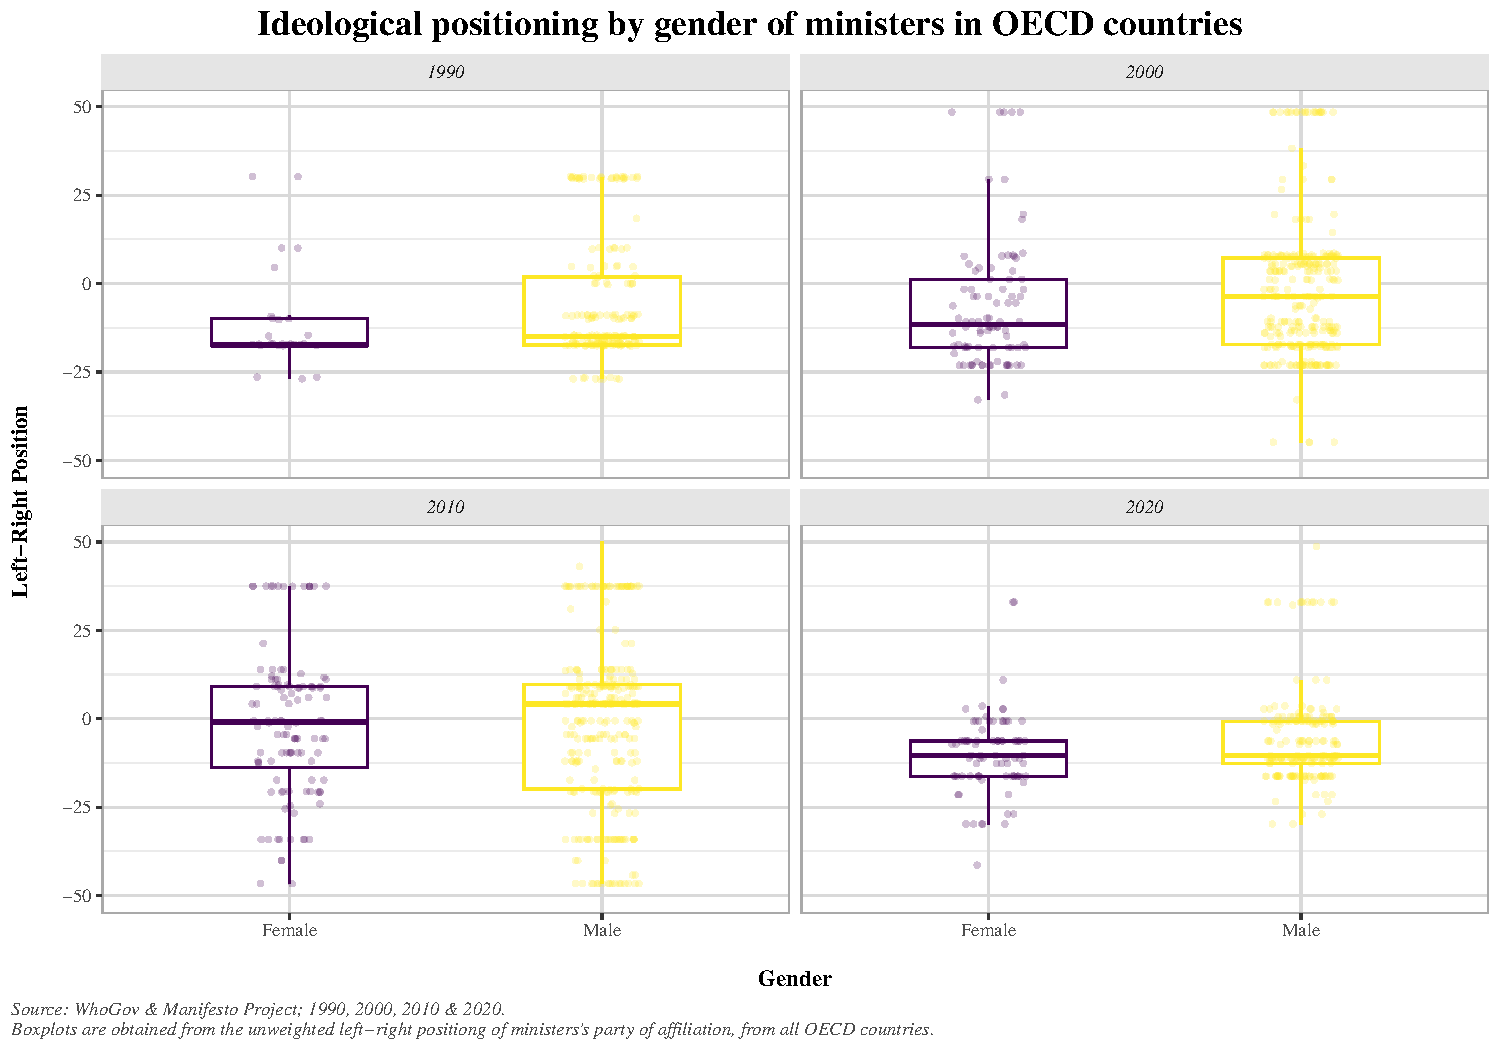
\includegraphics[width=1.1\textwidth]{boxplot_gender.pdf}
\end{figure}

\vspace{0.5cm}
\noindent In all the years analysed, the mean ideological positioning of female ministers is more left-leaning than that of their male counterparts, with only a minimal difference in 1990 and 2020. The boxplots for men show a more spread distribution, with a higher number of observations outside the box boundaries. Notably, in 1990 the first quartile of men and women is at the same level (\emph{around -15}), and in 2010 the first quartile of men is more left-leaning than that of women, while their top quartiles are at the same level (\emph{around 10}). 

\noindent Overall, while Figure 5 suggests that women tend to have, on average, a more left-leaning ideological positioning than men, this pattern is not clearly reflected across the entire distribution.

\vspace{0.5cm}
\subsection{Heatplot of Within Cabinet Gender\-Gap in Ideology}

\vspace{0.5cm}
\noindent Lastly, as was mentioned in the stating of the hypothesis, women tend to position themselves more left on the ideological spectrum that their male counterparts within the ideological side. To test this claim a heatmap is constructed, considering the gap between female and male ministers in the same cabinet. 

\vspace{0.5cm}
\lstinputlisting[language=R, firstline=530, lastline=537]{final_MT.R}

\vspace{0.5cm}
\noindent To compute \textbf{gender\_gap} the observations are grouped by country, year and gender; afterwards, the average left-right ideological positioning is compted. The gender gap is calculated as the difference between the average RILE score of female and male ministers (\emph{female - male}). Since lower RILE scores indicate more left-leaning ideological positions, negative values of the gender gap imply that female ministers are, on average, more left-leaning than their male counterparts.

\noindent Some of the gender-gaps are not computable either because the RILE score for certain parties was not present or because only one of the two genders was present in the cabinet. 

\vspace{0.5cm}
\lstinputlisting[language=R, firstline=540, lastline=558]{final_MT.R}

\begin{figure}[H]\centering
	\caption{}
	\label{fig:visualisation_6}
	\hspace*{-1cm}
	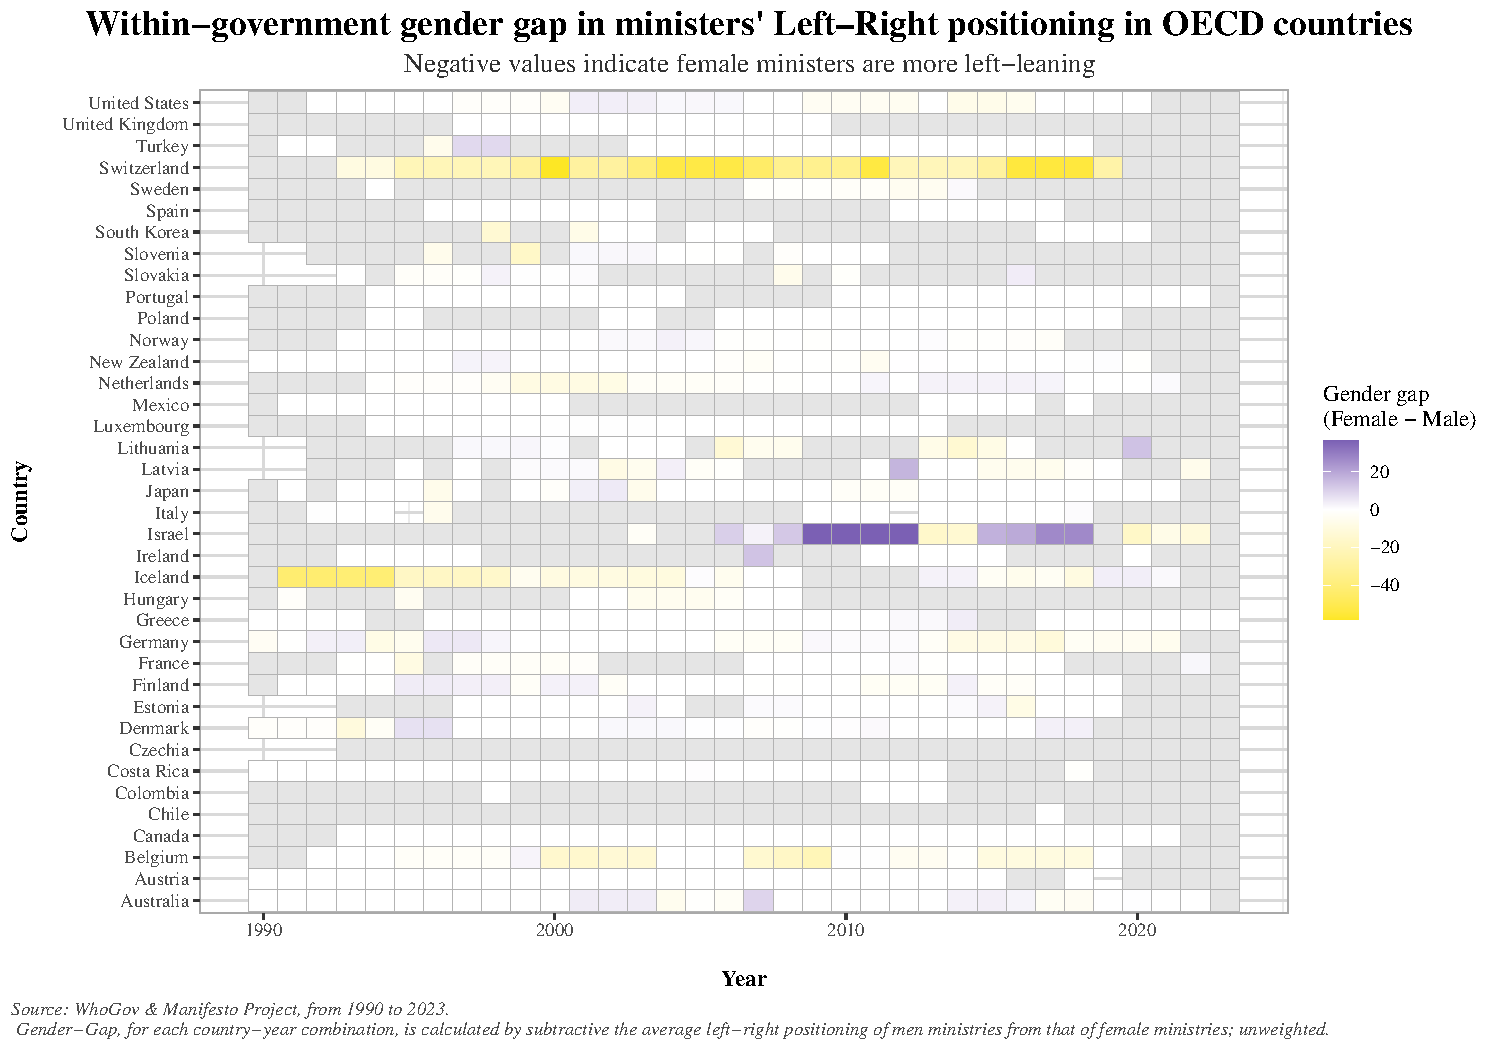
\includegraphics[width=1.1\textwidth]{heatmap_gender.pdf}
\end{figure}

\vspace{0.5cm}
\noindent While most of the map appears in a white, or adjacent, shade, some colours can still be observed and analysed. With the notable exception of \emph{Israel}, where female ministers appear to be strongly more right-leaning than their male counterparts from 2009 to 2019, the coloured rectangles tend to appear more often in yellow shades. 

\noindent Nonetheless, the gender gap in ideology within cabinets does not appear to be constant across OECD countries, with most country-year combinations being neutral and closer to 0, indicating only limited ideological differences between female and male ministers.

\vspace{0.5cm}

\section{Conclusion}

\vspace{0.5cm}

\noindent The visualisations presented in this report suggest only a weak relationship between the gender of politicians and their left-right ideological positioning. Overall, the analysis does not provide strong evidence of a systematic association between these two variables.

\noindent Figures 1 to 4 do not show a meaningful change in the average RILE positioning of cabinets as the share of female ministers increases, contrary to what was expected based on the initial hypothesis. Although the mean ideological positioning of female politicians often appears slightly more left-leaning than that of their male counterparts, this pattern does not consistently extend to the full distribution of observations. Male ministers generally display a more dispersed distribution, which occasionally results in more left-leaning scores for certain quartiles.

\noindent Finally, the heatmap does not reveal a stable or consistent gender gap in ideology within cabinets across OECD countries and years. Taken together, these findings suggest that ideological differences between male and female ministers are limited and may depend more strongly on country-specific political contexts rather than gender alone.

	
\end{document}